% Options for packages loaded elsewhere
\PassOptionsToPackage{unicode}{hyperref}
\PassOptionsToPackage{hyphens}{url}
\PassOptionsToPackage{dvipsnames,svgnames,x11names}{xcolor}
%
\documentclass[
  letterpaper,
  DIV=11,
  numbers=noendperiod]{scrreprt}

\usepackage{amsmath,amssymb}
\usepackage{iftex}
\ifPDFTeX
  \usepackage[T1]{fontenc}
  \usepackage[utf8]{inputenc}
  \usepackage{textcomp} % provide euro and other symbols
\else % if luatex or xetex
  \usepackage{unicode-math}
  \defaultfontfeatures{Scale=MatchLowercase}
  \defaultfontfeatures[\rmfamily]{Ligatures=TeX,Scale=1}
\fi
\usepackage{lmodern}
\ifPDFTeX\else  
    % xetex/luatex font selection
\fi
% Use upquote if available, for straight quotes in verbatim environments
\IfFileExists{upquote.sty}{\usepackage{upquote}}{}
\IfFileExists{microtype.sty}{% use microtype if available
  \usepackage[]{microtype}
  \UseMicrotypeSet[protrusion]{basicmath} % disable protrusion for tt fonts
}{}
\makeatletter
\@ifundefined{KOMAClassName}{% if non-KOMA class
  \IfFileExists{parskip.sty}{%
    \usepackage{parskip}
  }{% else
    \setlength{\parindent}{0pt}
    \setlength{\parskip}{6pt plus 2pt minus 1pt}}
}{% if KOMA class
  \KOMAoptions{parskip=half}}
\makeatother
\usepackage{xcolor}
\setlength{\emergencystretch}{3em} % prevent overfull lines
\setcounter{secnumdepth}{5}
% Make \paragraph and \subparagraph free-standing
\ifx\paragraph\undefined\else
  \let\oldparagraph\paragraph
  \renewcommand{\paragraph}[1]{\oldparagraph{#1}\mbox{}}
\fi
\ifx\subparagraph\undefined\else
  \let\oldsubparagraph\subparagraph
  \renewcommand{\subparagraph}[1]{\oldsubparagraph{#1}\mbox{}}
\fi

\usepackage{color}
\usepackage{fancyvrb}
\newcommand{\VerbBar}{|}
\newcommand{\VERB}{\Verb[commandchars=\\\{\}]}
\DefineVerbatimEnvironment{Highlighting}{Verbatim}{commandchars=\\\{\}}
% Add ',fontsize=\small' for more characters per line
\usepackage{framed}
\definecolor{shadecolor}{RGB}{241,243,245}
\newenvironment{Shaded}{\begin{snugshade}}{\end{snugshade}}
\newcommand{\AlertTok}[1]{\textcolor[rgb]{0.68,0.00,0.00}{#1}}
\newcommand{\AnnotationTok}[1]{\textcolor[rgb]{0.37,0.37,0.37}{#1}}
\newcommand{\AttributeTok}[1]{\textcolor[rgb]{0.40,0.45,0.13}{#1}}
\newcommand{\BaseNTok}[1]{\textcolor[rgb]{0.68,0.00,0.00}{#1}}
\newcommand{\BuiltInTok}[1]{\textcolor[rgb]{0.00,0.23,0.31}{#1}}
\newcommand{\CharTok}[1]{\textcolor[rgb]{0.13,0.47,0.30}{#1}}
\newcommand{\CommentTok}[1]{\textcolor[rgb]{0.37,0.37,0.37}{#1}}
\newcommand{\CommentVarTok}[1]{\textcolor[rgb]{0.37,0.37,0.37}{\textit{#1}}}
\newcommand{\ConstantTok}[1]{\textcolor[rgb]{0.56,0.35,0.01}{#1}}
\newcommand{\ControlFlowTok}[1]{\textcolor[rgb]{0.00,0.23,0.31}{#1}}
\newcommand{\DataTypeTok}[1]{\textcolor[rgb]{0.68,0.00,0.00}{#1}}
\newcommand{\DecValTok}[1]{\textcolor[rgb]{0.68,0.00,0.00}{#1}}
\newcommand{\DocumentationTok}[1]{\textcolor[rgb]{0.37,0.37,0.37}{\textit{#1}}}
\newcommand{\ErrorTok}[1]{\textcolor[rgb]{0.68,0.00,0.00}{#1}}
\newcommand{\ExtensionTok}[1]{\textcolor[rgb]{0.00,0.23,0.31}{#1}}
\newcommand{\FloatTok}[1]{\textcolor[rgb]{0.68,0.00,0.00}{#1}}
\newcommand{\FunctionTok}[1]{\textcolor[rgb]{0.28,0.35,0.67}{#1}}
\newcommand{\ImportTok}[1]{\textcolor[rgb]{0.00,0.46,0.62}{#1}}
\newcommand{\InformationTok}[1]{\textcolor[rgb]{0.37,0.37,0.37}{#1}}
\newcommand{\KeywordTok}[1]{\textcolor[rgb]{0.00,0.23,0.31}{#1}}
\newcommand{\NormalTok}[1]{\textcolor[rgb]{0.00,0.23,0.31}{#1}}
\newcommand{\OperatorTok}[1]{\textcolor[rgb]{0.37,0.37,0.37}{#1}}
\newcommand{\OtherTok}[1]{\textcolor[rgb]{0.00,0.23,0.31}{#1}}
\newcommand{\PreprocessorTok}[1]{\textcolor[rgb]{0.68,0.00,0.00}{#1}}
\newcommand{\RegionMarkerTok}[1]{\textcolor[rgb]{0.00,0.23,0.31}{#1}}
\newcommand{\SpecialCharTok}[1]{\textcolor[rgb]{0.37,0.37,0.37}{#1}}
\newcommand{\SpecialStringTok}[1]{\textcolor[rgb]{0.13,0.47,0.30}{#1}}
\newcommand{\StringTok}[1]{\textcolor[rgb]{0.13,0.47,0.30}{#1}}
\newcommand{\VariableTok}[1]{\textcolor[rgb]{0.07,0.07,0.07}{#1}}
\newcommand{\VerbatimStringTok}[1]{\textcolor[rgb]{0.13,0.47,0.30}{#1}}
\newcommand{\WarningTok}[1]{\textcolor[rgb]{0.37,0.37,0.37}{\textit{#1}}}

\providecommand{\tightlist}{%
  \setlength{\itemsep}{0pt}\setlength{\parskip}{0pt}}\usepackage{longtable,booktabs,array}
\usepackage{calc} % for calculating minipage widths
% Correct order of tables after \paragraph or \subparagraph
\usepackage{etoolbox}
\makeatletter
\patchcmd\longtable{\par}{\if@noskipsec\mbox{}\fi\par}{}{}
\makeatother
% Allow footnotes in longtable head/foot
\IfFileExists{footnotehyper.sty}{\usepackage{footnotehyper}}{\usepackage{footnote}}
\makesavenoteenv{longtable}
\usepackage{graphicx}
\makeatletter
\def\maxwidth{\ifdim\Gin@nat@width>\linewidth\linewidth\else\Gin@nat@width\fi}
\def\maxheight{\ifdim\Gin@nat@height>\textheight\textheight\else\Gin@nat@height\fi}
\makeatother
% Scale images if necessary, so that they will not overflow the page
% margins by default, and it is still possible to overwrite the defaults
% using explicit options in \includegraphics[width, height, ...]{}
\setkeys{Gin}{width=\maxwidth,height=\maxheight,keepaspectratio}
% Set default figure placement to htbp
\makeatletter
\def\fps@figure{htbp}
\makeatother
\newlength{\cslhangindent}
\setlength{\cslhangindent}{1.5em}
\newlength{\csllabelwidth}
\setlength{\csllabelwidth}{3em}
\newlength{\cslentryspacingunit} % times entry-spacing
\setlength{\cslentryspacingunit}{\parskip}
\newenvironment{CSLReferences}[2] % #1 hanging-ident, #2 entry spacing
 {% don't indent paragraphs
  \setlength{\parindent}{0pt}
  % turn on hanging indent if param 1 is 1
  \ifodd #1
  \let\oldpar\par
  \def\par{\hangindent=\cslhangindent\oldpar}
  \fi
  % set entry spacing
  \setlength{\parskip}{#2\cslentryspacingunit}
 }%
 {}
\usepackage{calc}
\newcommand{\CSLBlock}[1]{#1\hfill\break}
\newcommand{\CSLLeftMargin}[1]{\parbox[t]{\csllabelwidth}{#1}}
\newcommand{\CSLRightInline}[1]{\parbox[t]{\linewidth - \csllabelwidth}{#1}\break}
\newcommand{\CSLIndent}[1]{\hspace{\cslhangindent}#1}

\KOMAoption{captions}{tableheading}
\makeatletter
\makeatother
\makeatletter
\@ifpackageloaded{bookmark}{}{\usepackage{bookmark}}
\makeatother
\makeatletter
\@ifpackageloaded{caption}{}{\usepackage{caption}}
\AtBeginDocument{%
\ifdefined\contentsname
  \renewcommand*\contentsname{Table of contents}
\else
  \newcommand\contentsname{Table of contents}
\fi
\ifdefined\listfigurename
  \renewcommand*\listfigurename{List of Figures}
\else
  \newcommand\listfigurename{List of Figures}
\fi
\ifdefined\listtablename
  \renewcommand*\listtablename{List of Tables}
\else
  \newcommand\listtablename{List of Tables}
\fi
\ifdefined\figurename
  \renewcommand*\figurename{Figure}
\else
  \newcommand\figurename{Figure}
\fi
\ifdefined\tablename
  \renewcommand*\tablename{Table}
\else
  \newcommand\tablename{Table}
\fi
}
\@ifpackageloaded{float}{}{\usepackage{float}}
\floatstyle{ruled}
\@ifundefined{c@chapter}{\newfloat{codelisting}{h}{lop}}{\newfloat{codelisting}{h}{lop}[chapter]}
\floatname{codelisting}{Listing}
\newcommand*\listoflistings{\listof{codelisting}{List of Listings}}
\makeatother
\makeatletter
\@ifpackageloaded{caption}{}{\usepackage{caption}}
\@ifpackageloaded{subcaption}{}{\usepackage{subcaption}}
\makeatother
\makeatletter
\@ifpackageloaded{tcolorbox}{}{\usepackage[skins,breakable]{tcolorbox}}
\makeatother
\makeatletter
\@ifundefined{shadecolor}{\definecolor{shadecolor}{rgb}{.97, .97, .97}}
\makeatother
\makeatletter
\makeatother
\makeatletter
\makeatother
\ifLuaTeX
  \usepackage{selnolig}  % disable illegal ligatures
\fi
\IfFileExists{bookmark.sty}{\usepackage{bookmark}}{\usepackage{hyperref}}
\IfFileExists{xurl.sty}{\usepackage{xurl}}{} % add URL line breaks if available
\urlstyle{same} % disable monospaced font for URLs
\hypersetup{
  pdftitle={Learning diary},
  pdfauthor={Lama Alswliman},
  colorlinks=true,
  linkcolor={blue},
  filecolor={Maroon},
  citecolor={Blue},
  urlcolor={Blue},
  pdfcreator={LaTeX via pandoc}}

\title{Learning diary}
\author{Lama Alswliman}
\date{2026-06-01}

\begin{document}
\maketitle
\ifdefined\Shaded\renewenvironment{Shaded}{\begin{tcolorbox}[interior hidden, boxrule=0pt, sharp corners, breakable, frame hidden, enhanced, borderline west={3pt}{0pt}{shadecolor}]}{\end{tcolorbox}}\fi

\renewcommand*\contentsname{Table of contents}
{
\hypersetup{linkcolor=}
\setcounter{tocdepth}{2}
\tableofcontents
}
\bookmarksetup{startatroot}

\hypertarget{about}{%
\chapter*{About}\label{about}}
\addcontentsline{toc}{chapter}{About}

\markboth{About}{About}

\bookmarksetup{startatroot}

\hypertarget{week-1-remote-sensing-an-arial-adventure}{%
\chapter{Week 1 Remote sensing: an Arial
adventure}\label{week-1-remote-sensing-an-arial-adventure}}

\hypertarget{summary}{%
\section{Summary}\label{summary}}

In this lecture, we delved into the world of remotely sensing cities,
and learned about the methods used to collect data using sensors that
are mounted on various of platforms (spaceborne/airborne). We explored
the two main types of sensors: passive, which detect natural radiation,
and active, which emit their own radiation. We also explored the
differences between Sentinel 2 and Landsat satellites in terms of
spectral bands, spatial resolution, and revisit frequency. Finally, we
discussed that electromagnetic radiation can be obstructed by surfaces
or the atmosphere, causing absorption, transmission, or scattering.

\begin{figure}

{\centering 

\href{https://www.balamis.com/technology/}{\includegraphics[width=5.20833in,height=\textheight]{active and passive sensors .gif}}

}

\caption{Figure (1): Active and Passive sensors. website:
(https://www.balamis.com/technology/)}

\end{figure}

\hypertarget{remote-sensing-definition}{%
\subsection{Remote sensing definition}\label{remote-sensing-definition}}

According to NASA ``Remote sensing is the acquiring of information from
a distance''. By observing the energy response (reflected, transmitted)
and recording information then use it in responding to hazards, apply
energy studies utilizing, urban planning, and environmental treaty
enforcement\ldots..etc.

\hypertarget{the-process-of-remote-sensing}{%
\subsection{The process of remote
sensing}\label{the-process-of-remote-sensing}}

Electromagnetic energy, created by moving charged particles, travels in
waves through space and the atmosphere. These waves vary in length and
frequency; shorter waves have higher frequencies. Electromagnetic waves
might get obstructed by a surface or atmosphere which cause scattering
for the short wave such as blues and then it reflects back to be
recorded and processed to information/data.

\begin{figure}

{\centering 

\href{https://paititi.info/research-technology/remote-sensing-from-space/}{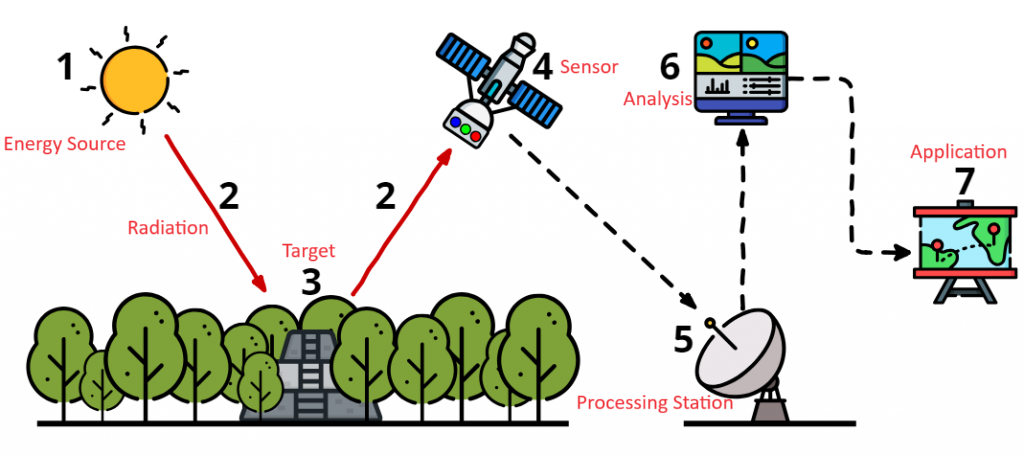
\includegraphics[width=5.20833in,height=\textheight]{4-1-Remote-Sensing-Process-1024x455.png}}

}

\caption{Figure (2): the remote sensing process website:
(https://paititi.info/research-technology/remote-sensing-from-space/)}

\end{figure}

\hypertarget{sentinel-2-vs-landsat}{%
\subsection{Sentinel-2 VS Landsat}\label{sentinel-2-vs-landsat}}

\textbf{Sentinel-2} The SENTINEL-2 mission consists of two satellites
orbiting in the same path around the Earth, but spaced 180° apart.
They're designed to continuously observe changes in land surface
conditions. With a wide coverage area and a rapid revisit time of 10
days at the equator.

\textbf{Landsat 8} The Landsat 8 satellite carries two main instruments:
the Operational Land Imager (OLI) and the Thermal Infrared Sensor
(TIRS). These sensors capture images of the Earth's surface at various
resolutions, including 30 meters for visible, near-infrared, and
short-wave infrared data; 100 meters for thermal data; and 15 meters for
panchromatic data

\hypertarget{application}{%
\section{Application}\label{application}}

Landsat and Sentinel 2 have been used extensively in different fields
including land use planning and monitoring, emergency response and
management, water use monitoring and others. Each one of those two
methods has its strengths and to understand those strengths, we will
leverage an analysis that was conducted to evaluate and compare between
those two data sources in forest fires mapping article. This analysis
compares and assesses spectral indices derived from Sentinel-2 and
Landsat-8 OLI imagery and to identify the most appropriate iindex for
each sensor for accurately mapping forest fires, using as a case study
two fire events that occurred in summer 2017 in northern Tunisia (Achour
et al.~2022, Toujani et al.~2022).

\begin{figure}

{\centering 

\href{https://earthexplorer.usgs.gov/}{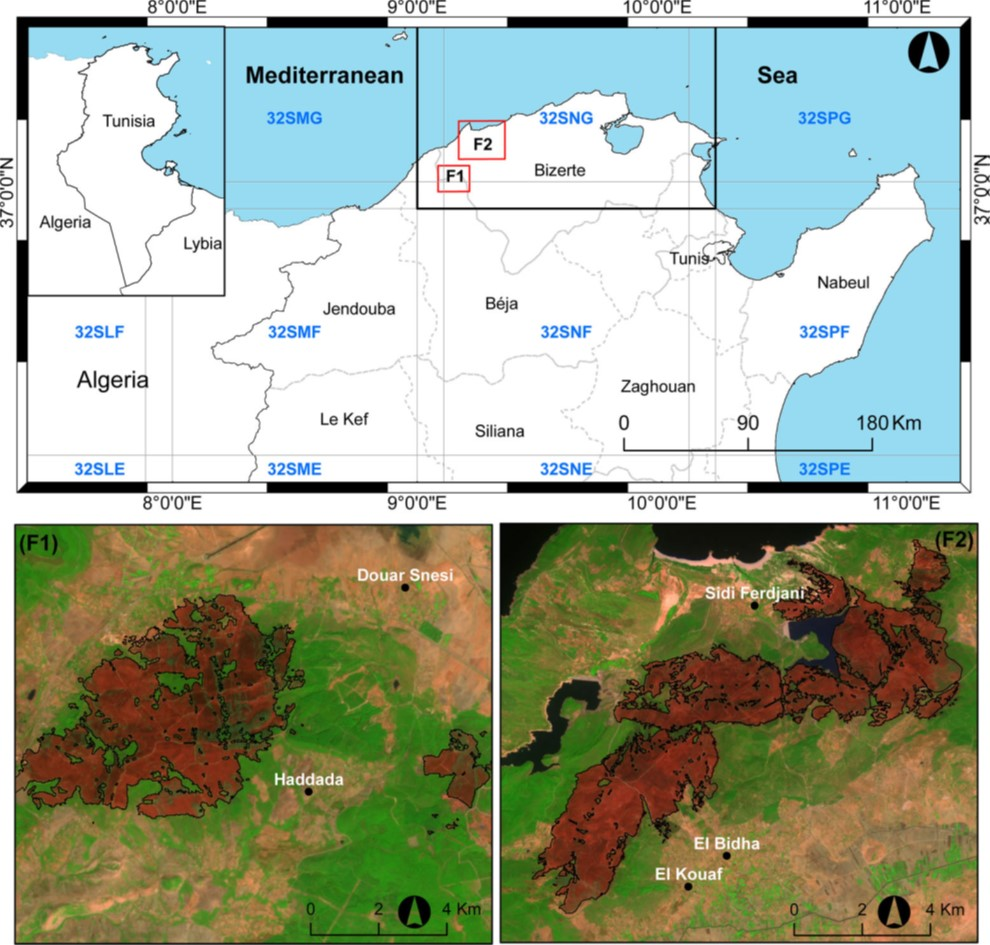
\includegraphics[width=5.20833in,height=\textheight]{application 1.jpg}}

}

\caption{Figure (2): Sentinel 2A Multi Spectral Instrument (MSI) and
Landsat-8 Operational Land Imager (OLI) satellite images were acquired
before (pre-fire) and after (post-fire) the fires from the U.S.
Geological Survey (USGS) website (https://earthexplorer.usgs.gov/).}

\end{figure}

\hypertarget{discussion}{%
\subsection{Discussion}\label{discussion}}

Results from this study highlight those spectral indices including
NIR-SWIR bands derived from Landsat 8 OLI and Sentinel-2 MSI (ΔNBRn,
ΔNBR and RBR) had higher discriminatory power than classical indices
based on NIR and red bands (BAI, ΔNDVI, ΔEVI, and ΔMSAVI).

In the figure below, we can see that spectral indices derived from
Landsat 8, especially those combining the Red-NIR bands such as ΔNDVI,
ΔEVI and ΔMSAVI exhibited a higher spectral separability as compared to
their counterparts generated from Sentinel bands in both fires.

\begin{figure}

{\centering 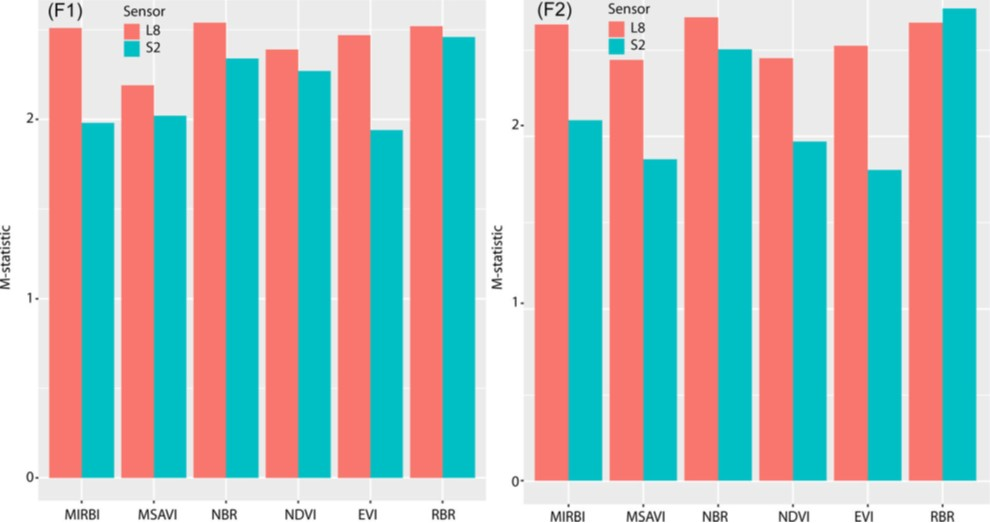
\includegraphics[width=5.20833in,height=\textheight]{application2.jpg}

}

\caption{Figure (3): M-statistic values to discern burned/unburned areas
for both Sentinel 2 (S) and Landsat-8 OLI (L) spectral indices}

\end{figure}

Maps of the estimated burned areas from each spectral index and for each
fire reveals that both Landsat 8 and Sentinel-2A can capture the
boundaries of fires identified using Copernicus EMS reference maps,
albeit with small differences between burned areas, retrieved from each
sensor.

Sentinel-based spectral indices (ΔNBRn and RBR) provided the highest
level of positional accuracy, with a loc value of about 60 metres. This
means that the positions of the extracted fires were shifted
approximately by three pixels from their positions in the reference map.
However, Landsat-based spectral indices, RBR and ΔNBR, displayed a loc
value of about 75 meters, suggesting that the position of the extracted
fires were shifted approximately 2.5 pixels from their positions in the
reference map. The advantage of Sentinel 2A in terms of positional
accuracy could be attributed to its higher spatial resolution as
compared to Landsat 8.

\begin{figure}

{\centering 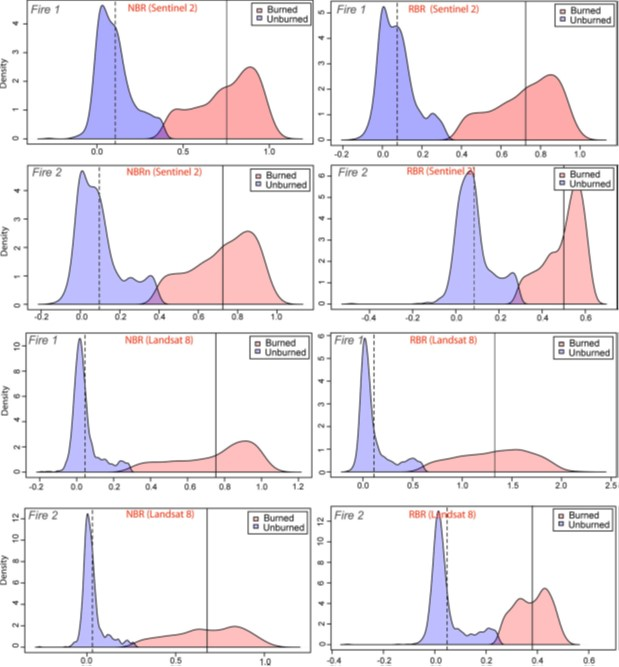
\includegraphics[width=5.20833in,height=\textheight]{application 3.jpg}

}

\caption{Figure (4): Distribution of burned and unburned values for
spectral indices selected for F1 / F2}

\end{figure}

\begin{figure}

{\centering 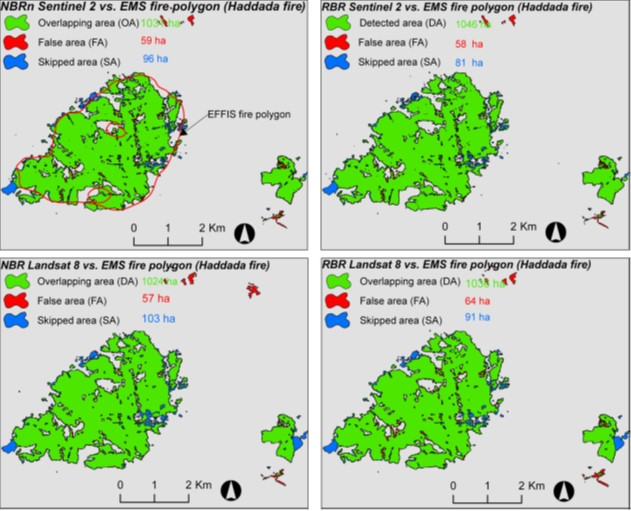
\includegraphics[width=5.20833in,height=\textheight]{application 4.jpg}

}

\caption{Figure (5): Spectral indices vs.~Copernicus EMS fire polygon
for the Haddada fire}

\end{figure}

\hypertarget{conclusion}{%
\subsection{Conclusion}\label{conclusion}}

The study concluded that (1) regardless of the sensor, spectral indices
that incorporated NIR-SWIR bands exceed those using red and NIR bands in
terms of spectral separability; (2) from the viewpoint of accuracy, the
Sentinel sensor is slightly more efficient than the Landsat 8 in mapping
burned scars, but both sensors produce similar and acceptable results.
Hence, this paper concludes that both sensors are a good alternative to
EFFIS data, particularly when there is a need to detect details inside
the fire. \textbf{I still have to add so what and why it is useful:}

\hypertarget{reflection}{%
\section{Reflection}\label{reflection}}

This lecture wasn't easy to digest \textbf{\emph{at first,}} as there
was a lot of new ideas and terms (Spectral, Spectrum, Spectral
Signature\ldots etc ) to learn. when I went through the lecture it was
captivating the facts that we learned for example the scattering of EMR
and how the process of gathering satellite images is not as easy and
simple as i thought, plus it was really interesting knowing why the sky
and sea are blue. This lecture opened my eyes to the uses of satellite
data and the importance of it and how it can be used in different areas
and in very different methods but what was really interesting for me is
the paper that i found on the use of satellite images in capturing the
socioeconomic disruption during the Ukrainian war. In this study they
combined satellite data on nitrogen dioxide (NO2) and carbon dioxide
(CO2) to track changes in human activities, as both gases are linked to
fossil fuel combustion. the analysis reveals a significant decrease in
NO2 levels over major Ukrainian cities, power plants, and industrial
areas during the second quarter of 2022, ranging from 15\% to 46\%
compared to the reference period of 2018-2021. They also used the
detection of unusual fire which might be likley from shelling rather
than agricultural burning.These findings demonstrate the value of
satellite observations in monitoring significant societal changes,
particularly during conflicts.

\bookmarksetup{startatroot}

\hypertarget{references}{%
\chapter*{References}\label{references}}
\addcontentsline{toc}{chapter}{References}

\markboth{References}{References}

Evaluation and comparison of Sentinel-2 MSI, Landsat 8 OLI, and EFFIS
data for forest fires mapping. Illustrations from the summer 2017 fires
in Tunisia.

\url{https://www.tandfonline.com/doi/full/10.1080/10106049.2021.1980118}

\bookmarksetup{startatroot}

\hypertarget{introduction}{%
\chapter{Introduction}\label{introduction}}

This is a book created from markdown and executable code.

See Knuth (1984) for additional discussion of literate programming.

\begin{Shaded}
\begin{Highlighting}[]
\DecValTok{1} \SpecialCharTok{+} \DecValTok{1}
\end{Highlighting}
\end{Shaded}

\begin{verbatim}
[1] 2
\end{verbatim}

\bookmarksetup{startatroot}

\hypertarget{summary-1}{%
\chapter{Summary}\label{summary-1}}

In summary, this book has no content whatsoever.

\begin{Shaded}
\begin{Highlighting}[]
\DecValTok{1} \SpecialCharTok{+} \DecValTok{1}
\end{Highlighting}
\end{Shaded}

\begin{verbatim}
[1] 2
\end{verbatim}

\bookmarksetup{startatroot}

\hypertarget{references-1}{%
\chapter*{References}\label{references-1}}
\addcontentsline{toc}{chapter}{References}

\markboth{References}{References}

\hypertarget{refs}{}
\begin{CSLReferences}{1}{0}
\leavevmode\vadjust pre{\hypertarget{ref-knuth84}{}}%
Knuth, Donald E. 1984. {``Literate Programming.''} \emph{Comput. J.} 27
(2): 97--111. \url{https://doi.org/10.1093/comjnl/27.2.97}.

\end{CSLReferences}



\end{document}
